\section{Building Path Conditions}
\label{sec:building_pcs}

As well, we present our approach to building a set of path conditions to represent all executions of a DSLTrans transformation.



\subsection{Path Condition Generation Algorithm}
\label{sec:gen_all_pcs}

 This section will describe how path conditions are constructed for a DSLTrans transformation using our approach.

\cref{fig:next_layer} outlines the path condition generation algorithm. The algorithm will examine each transformation layer in turn. Path conditions from the previous layer will be combined with rules from the current layer to create a new set of path conditions. This new set of path conditions will then be combined with the rules from the next layer to produce yet another set of path conditions, and so on. At the end of the algorithm, a complete set of path conditions for the entire transformation will have been produced. 

\begin{figure*}[htb]
        \centering
        \begin{subfigure}[b]{0.34\textwidth}
                \centering
                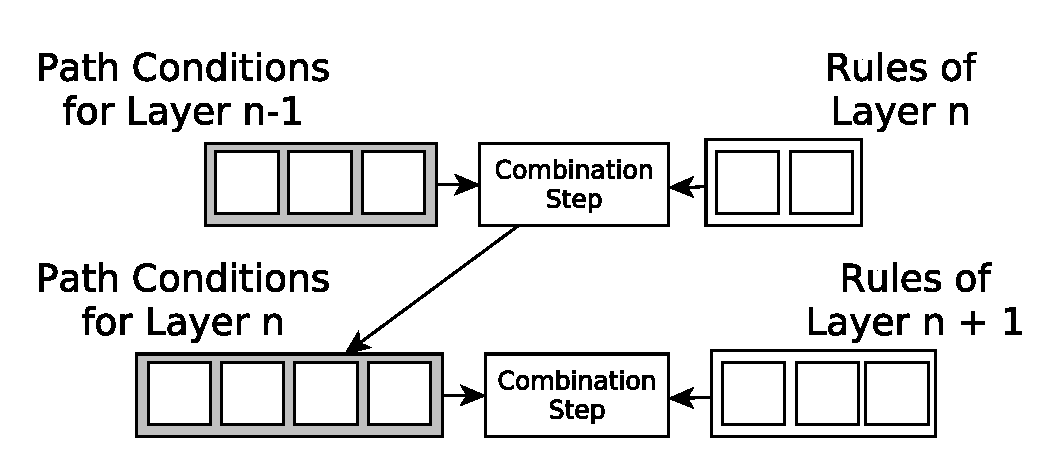
\includegraphics[width=1\textwidth]{./figures/building_path_conditions/next_layer.pdf}
                \caption{Previous path conditions are combined\\ with rules}
                \label{fig:next_layer}
        \end{subfigure}%
        ~~
        \begin{subfigure}[b]{0.34\textwidth}
                \centering
                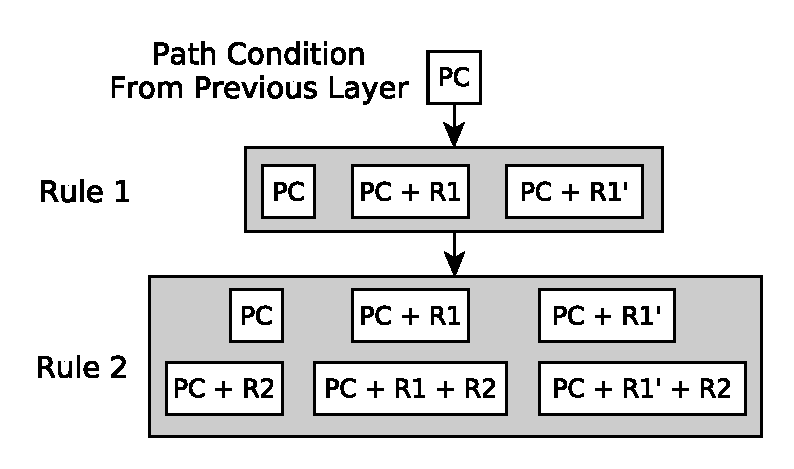
\includegraphics[width=1\textwidth]{./figures/overview/layers_pc.pdf}
                \caption{Combining a path condition with two rules\\~}
                \label{fig:layers_pc2}
        \end{subfigure}%
        
       
         \caption{Two components in the path condition creation process}
         \label{fig:combining_path_conditions}
\end{figure*}

We now define what is occurring in the `combination step' in \cref{fig:next_layer}. This step begins by selecting each path condition in the working set, one at a time. Note that at the beginning of the path condition creation process, this working set consists of an empty path condition.

A new set of path conditions will then be created by sequentially combining each rule in the layer with the path condition selected. Recall that a path condition represents a set of rules that have symbolically executed, thereby abstracting a set of transformation executions through our abstraction relation. \reviewer{we cannot recall this as it has not yet been presented;
the abstraction relation is defined only in Section 5}Combining a path condition with a rule will produce one or more path conditions depending on how the rule combines with the rules already represented by the path condition. The pre- and post- conditions defined by the path condition will be modified according to the elements found in that rule. 

Each of the new path conditions created from combining a rule with a path condition will then be combined with the next rule in the layer. A small example is shown in \cref{fig:layers_pc2}, where a path condition is combined with two rules. Note that a rule can combine with a path condition in multiple ways (differentiated by prime marks in the figure). \Cref{fig:all_pcs2} shows how path conditions from the previous layer are sequentially combined with all the rules from the current layer. All the path conditions for the layer are then collected to produce the final working set of path conditions for the layer.

        \begin{figure}[bht]
                 \centering
                  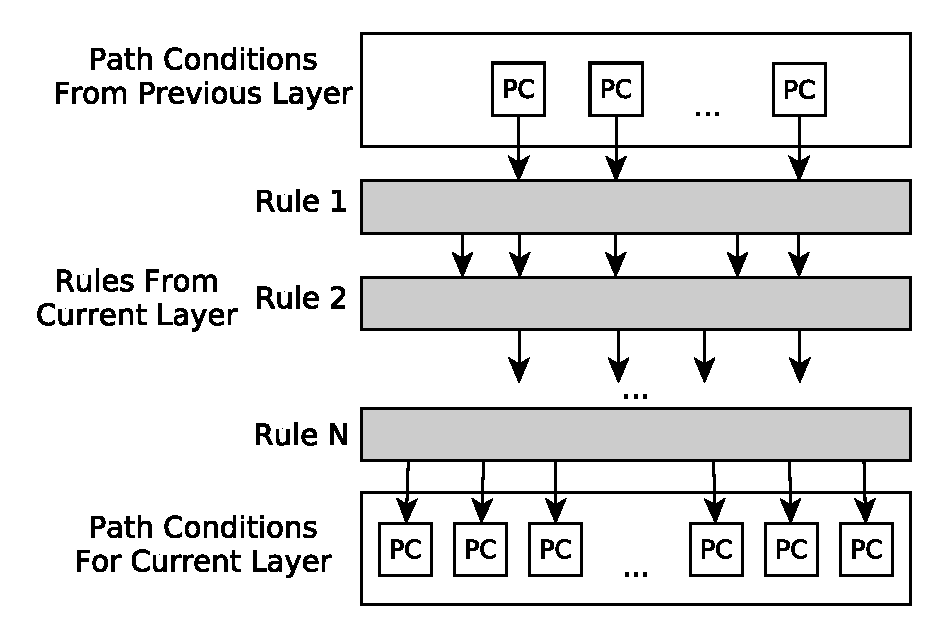
\includegraphics[width=.38\textwidth]{./figures/overview/all_pcs.pdf}
                 \caption{Creating all path conditions for a layer}
                 \label{fig:all_pcs2}
         \end{figure}
         
\subsection{Combining a Path Condition with a Rule}
We will now examine the combination step between one path condition and one rule, which produces a set of new path conditions. A formal and generic definition of this step will be presented first, before we explain the specialized combination possibilities with figures and informal text.

\begin{definition}{Combination of a Path Condition with a Rule}
\label{def:combine_pc_with_rule}

\reviewer{A $\sqcup$ operator is defined in Def. 19, but there you seem to
  rely on the fact that some elements of the path conditions and
  some elements of the rule are identical, otherwise the union
  would not work. Since a rule can be applied in several places,
  this would require a renaming of the rule elements, which - as 
  far as I could see - is not specified.}
  
Let $pc = \langle V',E',st',\tau',Match',Apply',Rulecop'\rangle\in\\
\textsc{Pathcond}^{sr}_{tg}$ be a path condition and $rl = \langle
V'',E'',st'',\tau'',\\Match'',Apply''\rangle\in \textsc{Rule}^{sr}_{tg}$ be a transformation rule, where their respective typed graphs can be joint. The union of $pc$ with $rl$ is built using the operator $\stackrel{trace}{\sqcup}:
\textsc{Pathcond}^{sr}_{tg}\times \textsc{Rule}^{sr}_{tg}\rightarrow
\textsc{Pathcond}^{sr}_{tg}$, as follows:

$$pc\stackrel{trace}{\sqcup}rl = \langle V,E,st,\tau,Match,Apply,Rulecop\rangle$$

where we have that $V=V'\cup V''$, $E'\cup E''\subseteq E$, $st'\cup
st''\subseteq st$, $\tau'\cup \tau''\subseteq \tau$ and if $v_1\xrightarrow{e}
v_2\in E\setminus E'\cup E''$ then we have that $v_1\in Apply(V'')$, $v_1\notin Apply(V')$, $v_2\in Match(V'')$ and also that $\tau'(e)=trace$. Additionally, $Match = Match'\sqcup Match''$ and $Apply = Apply'\sqcup Apply''$. Finally, we have that: $Rulecop = Rulecop'\cup$ {rl}.


% $$pc = \bigsqcup_{rl\in RC} trace(rl_{pathcond})$$
% 
% where $trace:\textsc{Pathcond}\rightarrow \textsc{Pathcond}$ is such that
% $trace(\langle V,E,st,\tau\rangle) = \langle V,E',st',\tau'\rangle$ and we have
% that: $E\subseteq E'$; $st\subseteq st'$; $\tau \subseteq \tau'$; if $\neg
% (v_1\xrightarrow{e'} v_2\in E)\;\land\;\tau(e')=backward$ then we have that if
% $v_1\in Apply(V)$ and $v_2\in Match(V)$ then $v_1\xrightarrow{e} v_2\in
% E'\setminus E$ and $\tau'(e)=trace$. Also, $rl_{pathcond}$ is rule $rl$ typed as
% a path condition by adding to the $rl$ tuple a $Rule$ function that identifies
% each vertex in $V$ as belonging to $rl$. Finally, we have used the
% $\sqcup$ notation to denote the extension of the typed graph union to the
% component-wise of tuples that represent path conditions.
\end{definition}

\reviewer{Def. 19 can only be understood once it is clear that your plan is to make iso-
morphic rule copies in which the node and edge identities already coincide with
those in your path condition. (Hence my “isomorphic representative” guess in
the previous remark.) This is very much nonstandard in the works of graph trans-
formation, and poorly motivated. What are the advantages of this approach over
relying on partial morphisms from a fixed rule to the path condition? As it is,
you have to explain that you only consider isomorphic copies that differ in rele-
vant parts, where “relevant” is determined by the question whether a node/edge
identity coincides with one on the path condition. (You actually do not explain
that at all: strictly following your definitions one would have to consider an in-
finite number of isomorphic rule copies, assuming that the number of available
identities is infinite (as it must be).)}

\reviewer{“joint” $\rightarrow$ “overlapping”? Why are the type graphs actually not
identical, as pc and rl are defined over the same source and target metamodels?
Last line: “rl” $\rightarrow$ “$\{rl\}$”}

\cref{def:combine_pc_with_rule} shows the formal definition of combining a path condition with a rule. When a path condition is combined with a rule their typed graphs are united. Additionally, symbolic traceability links will be built at this time between the newly added apply elements of the rule and all of the rule's match elements. As a reminder, the link creation algorithm and examples have been introduced in \cref{subsubsec:traceability}.\\

Note that the fact that the graphs are potentially joint allows us to overlap a rule with the path condition by anchoring the rule on traceability links shared by the path condition and the rule graph. In the mathematical development that follows we will often refer to the joint parts of two or more typed graphs using the term ``glue''.

We will now discuss the combination step possibilities. Let PC be the path condition selected from layer n-1, and R the rule selected from layer n. When PC and R are combined, there are four possibilities based on the dependencies between PC and R:

\begin{enumerate}
\item R has \textbf{no} dependencies
\item R has dependencies and \textbf{cannot} execute
\item R has dependencies and \textbf{may} execute
\item R has dependencies and \textbf{will} execute
\end{enumerate}

These dependencies are defined by the backward links within R. As mentioned in \cref{subsubsec:traceability}, backward links enforce that the elements in the apply graph were created by the connected elements in the match graph. In the context of combining a rule and a path condition, these backward links define dependencies between the rule and the elements created by the rules represented by the path condition. 

The figures below will demonstrate the four cases above. As a reminder of visual notation, the backward links are dashed lines between the match and apply graphs of the rule and path condition, while symbolic traceability links are solid lines between the two graphs.

\subsubsection{No Dependencies}
\label{enum:no_back}

The rule R has a match graph which represents its pre-conditions. For a particular transformation execution, it is possible that this match graph would not match a specific input model, and thus R would not execute in these transformation executions. To represent all such transformation executions where the rule R would not execute, PC is copied unchanged to the new set of path conditions.

To represent the transformation executions where the match graph of R would match, and therefore R would execute, a new path condition is produced which consists of the union between R and PC. This situation is
seen in \cref{fig:no_dependencies} and formally defined in \cref{def:rule_comb_no_dependencies}.

\begin{figure}[bt] \centering 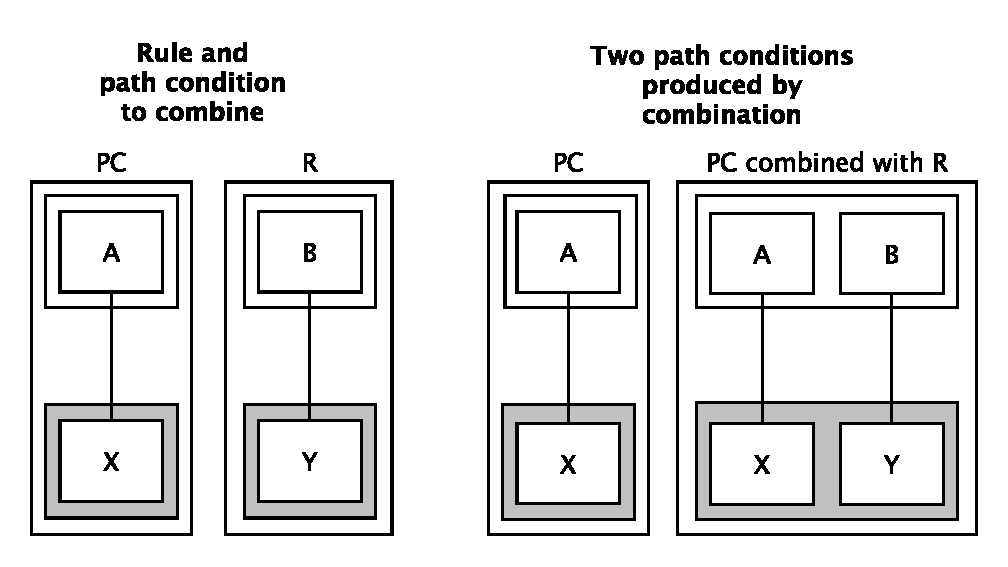
\includegraphics[width=0.44\textwidth]{./figures/building_path_conditions/no_dependencies.pdf}
	\caption{R has no dependencies}
	\label{fig:no_dependencies}
\end{figure}

% \begin{definition}{No Dependencies Between a Rule and a Path Condition}
% 
% \levi{FIX}
% Let $A=\langle V,E,st,\tau\rangle, B=\langle V',E',st',\tau'\rangle\in \textsc{Pathcond}^{sr}_{tg}$ be two path conditions. We say that $R$ does not depend on $PC$ if and only if $\nexists e\in E'\,.\,\tau'(e)=backward$.
% \end{definition}

\begin{definition}{Path Condition and Rule Combination -- No Dependencies\\}
\label{def:rule_comb_no_dependencies}

The combination of a path condition $pc$ and a rule $rl$, when $rl$ has no dependencies, is described by the relation $\stackrel{combine}{\rightarrow}\subseteq \textsc{Pathcond}^{sr}_{tg} \times \mathcal{P}(\textsc{Pathcond}^{sr}_{tg}) \times \textsc{Rule}^{sr}_{tg} \times \mathcal{P}(\textsc{Pathcond}^{sr}_{tg})$, defined as follows:	

% $$\frac{\begin{array}{ll}&
% pc\in PC\;,\;\langle pc,rl\rangle \xrightarrow{combine} pc'\;,\;PC\setminus\{pc\},rl,\rangle \xrightarrow{combstep} PC'
% \end{array}}
% {\langle PC,rules\rangle \xrightarrow{rulestep} PC'}$$

$$\frac{\begin{array}{ll}rl=\langle V,E,st,\tau, Match,Apply\big\rangle\;,\;\nexists e\in E\,.\,\tau'(e)=trace
\end{array}}
{\langle pc,AC,rl\rangle \xrightarrow{combine} AC\;\;\cup\;\; \bigcup_{pc'\in AC} pc'\stackrel{trace}{\sqcup} rl}$$

\end{definition}

\reviewer{The right hand side of the conclusion of Def. 20 has $AC \cup_{pc'\in AC} pc' $, of which
I cannot make sense. AC is a set, but the pc' are not, so what operation is
$\cup_{pc'\in AC} pc'$?}

\reviewer{Do you mean $\sqcup_{pc'\in AC}$instead? But then the result is not a set, so how can you take its union with AC? The same problem reoccurs in other definitions.}

Relation $\stackrel{combine}{\rightarrow}$ in \cref{def:rule_comb_no_dependencies} models the operational combination step shown in \cref{fig:layers_pc2} (the vertical black arrows between boxes). The relation has three input arguments: the first argument is the original path condition from the previous layer (shown as the topmost box in \cref{fig:layers_pc2} with label $PC$); the second argument is the set of path conditions accumulated thus far by combining other rules in the current layer with the original path condition; and the third argument is the rule from the current layer now being combined. The fourth argument of the relation, the relation's output, is the new set of path conditions resulting from this combination.

Briefly, the equation in \cref{def:rule_comb_no_dependencies} states that whenever a rule has no backward links typed as \emph{trace} (i.e. no dependencies), all path conditions in the accumulator set are kept, along with the result of combining all the path conditions in the accumulator set with the current rule. 

\subsubsection{Resolving Dependencies}
\label{subsubsec:resolve_dependencies}
If R contains backward links and thus R defines dependencies on PC, then we need to analyse whether PC can satisfy those dependencies. This is done by matching the backward links in R over the symbolic traceability links in PC. Note that symbolic traceability links in R are not required to be found in PC, and that only backward links define dependencies.

\paragraph{Unsatisfied Dependencies}


If the backward links in R cannot be matched to symbolic traceability links in PC, then in the transformation executions abstracted by PC, R cannot execute. Again, PC will be copied unchanged to the new set of path conditions, but no new path condition will be created. This case is shown in \cref{fig:non_satisfied_dependencies}, where the backward links between the two B elements in R cannot match over the symbolic traceability link in PC. \cref{def:rule_comb_unsatisfied} describes this case formally.

\begin{figure}[h!] \centering 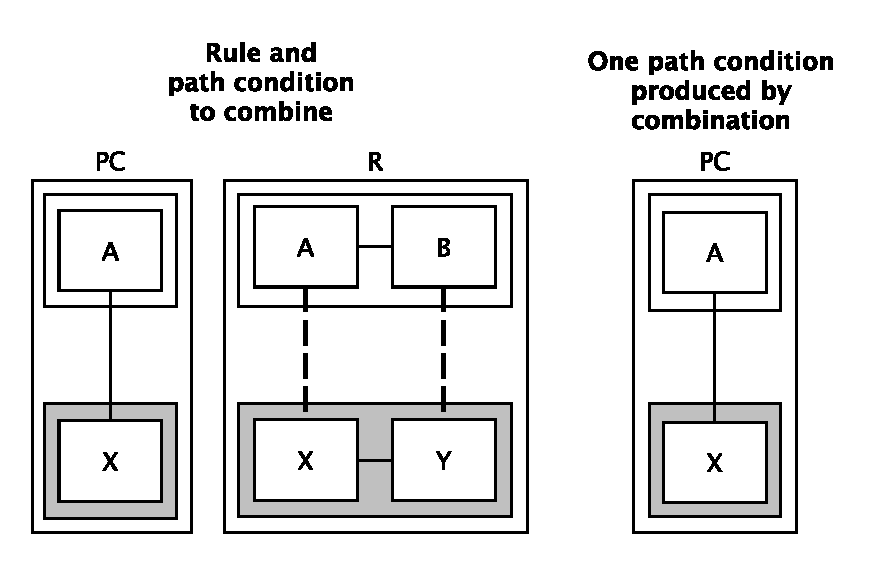
\includegraphics[width=0.44\textwidth]{./figures/building_path_conditions/non_satisfied_dependencies.pdf}
	\caption{R's dependencies are not satisfied by PC}
	\label{fig:non_satisfied_dependencies}
\end{figure}

\begin{definition}{Path Condition and Rule Combination -- Unsatisfied Dependencies\\} 
\label{def:rule_comb_unsatisfied}
% \begin{definition}{Unsatisfied Dependencies Between Two Path Conditions}
% 
% Let $A=\langle V_1,E_1,st_1,\tau_1\rangle, B=\langle V_2,E_2,st_2,\tau_2\rangle\in \textsc{Pathcond}^{sr}_{tg}$ be two path conditions. We say that $A$ does not satisfy $B$'s dependencies if and only if $\neg (B'\vartriangleleft A')$, where $A'=A_{|backward}$ and $B'=B_{|backward}$.
% \end{definition}



The combination of a path condition $pc$ and a rule $rl$, when $rl$ has dependencies that are not satisfied by $pc$, is described by the relation $\stackrel{combine}{\rightarrow}\subseteq \textsc{Pathcond}^{sr}_{tg}\times \mathcal{P}(\textsc{Pathcond}^{sr}_{tg})\\ \times \textsc{Rule}^{sr}_{tg} \times \mathcal{P}(\textsc{Pathcond}^{sr}_{tg})$, defined as follows:	

% $$\frac{\begin{array}{ll}&
% pc\in PC\;,\;\langle pc,rl\rangle \xrightarrow{combine} pc'\;,\;PC\setminus\{pc\},rl,\rangle \xrightarrow{combstep} PC'
% \end{array}}
% {\langle PC,rules\rangle \xrightarrow{rulestep} PC'}$$

$$\frac{\begin{array}{ll}\neg\big(rl|_{trace}\blacktriangleleft pc|_{trace}\big) \end{array}}
{\langle pc,AC,rl\rangle \xrightarrow{combine} AC}$$

\end{definition}

According to the pre-conditions of the equation presented in \cref{def:rule_comb_unsatisfied}, a path condition does not satisfy the dependencies present in a rule if there is no surjective typed graph homomorphism between the backward links of the rule and the symbolic traceability links of the path condition. Besides expressing the fact that all backward links must exist as symbolic traceability links the path condition, the surjective homomorphism allows modeling the case where dependencies expressed by two (or more) backward links between similarly typed elements can be satisfied by one single symbolic traceability link in the path condition \reviewer{Could be rephrased}. This is the case, for example, of rule \emph{FemaleToFemale} in the \emph{Police Station} in \cref{fig:dsltransformation}. The two similarly typed backward links in this rule are satisfied by a path condition containing only the rule \emph{females} generated from the first layer of the transformation, holding one single symbolic traceability link.


\paragraph{Partially- and Totally- Satisfied Dependencies}

Consider the possibility that the backward links of R can be found in PC, and R's dependencies are met. The question then becomes whether the rule R \textbf{may} or \textbf{will} execute in the abstracted transformation executions.

To resolve this question, the match graph of R, along with R's backward links, is matched to PC's match graph and traceability links. If all of these elements are found, then we denote this as the `totally-satisfied case', where R \textbf{will} necessarily execute in the abstracted transformation executions. Otherwise, we denote the `partially-satisfied' case, where R \textbf{may} execute. Note that we break up these cases for ease of explanation only. Formally, both cases are encompassed by \cref{def:rul_comb_partial_total}.

In the totally-satisfied case, R will be ``glued'' overtop PC, as seen in \cref{fig:total_satisfied_dependencies}. This gluing operation is anchored where the backwards links in R match over the traceability links in PC. The purpose of this operation is to include any elements in R's apply graph that may not exist in PC. Thus, all elements and associations which exist in both PC and R are ignored. Note that if multiple total matches exist in PC, that R will be glued at multiple points as seen in \cref{fig:multiple_total_satisfied_dependencies}. This ``gluing'' operation is also defined formally in \cref{def:rul_comb_partial_total}, as the addition of a delta graph.

\begin{figure*}[htb]
        \centering
        \begin{subfigure}[b]{0.7\textwidth}
                \centering
                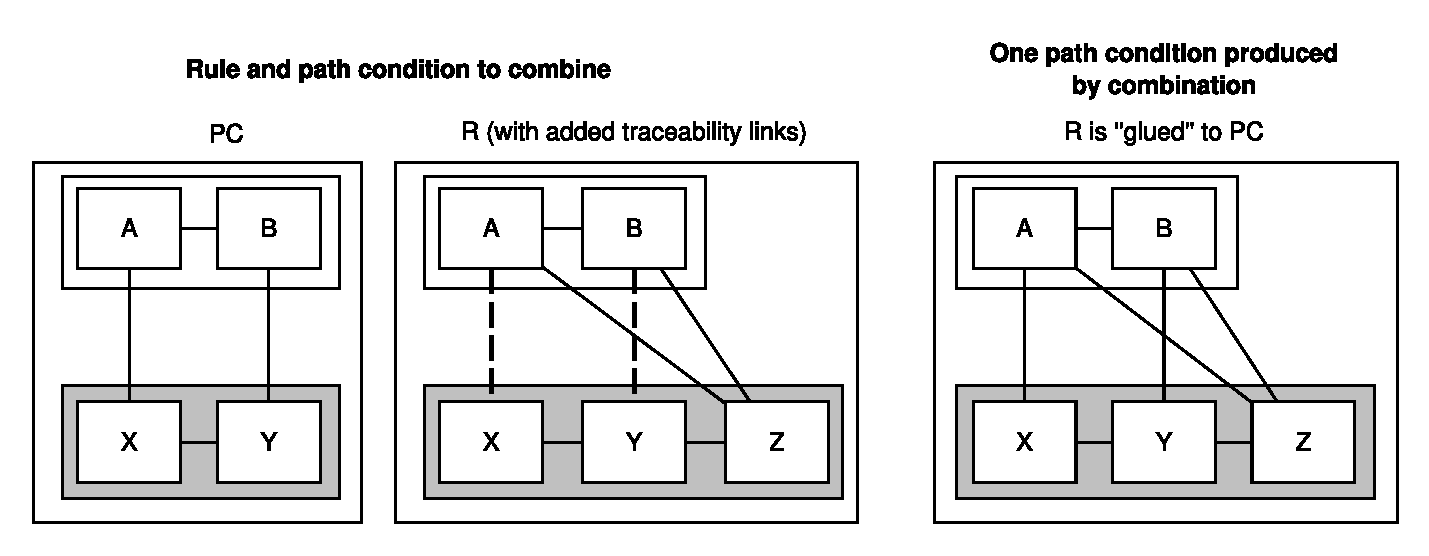
\includegraphics[width=1\textwidth]{./figures/building_path_conditions/total_satisfied_dependencies.pdf}
                \caption{Totally satisfied at one location}
                \label{fig:total_satisfied_dependencies}
        \end{subfigure}%
        \\
        \begin{subfigure}[b]{0.8\textwidth}
                \centering
                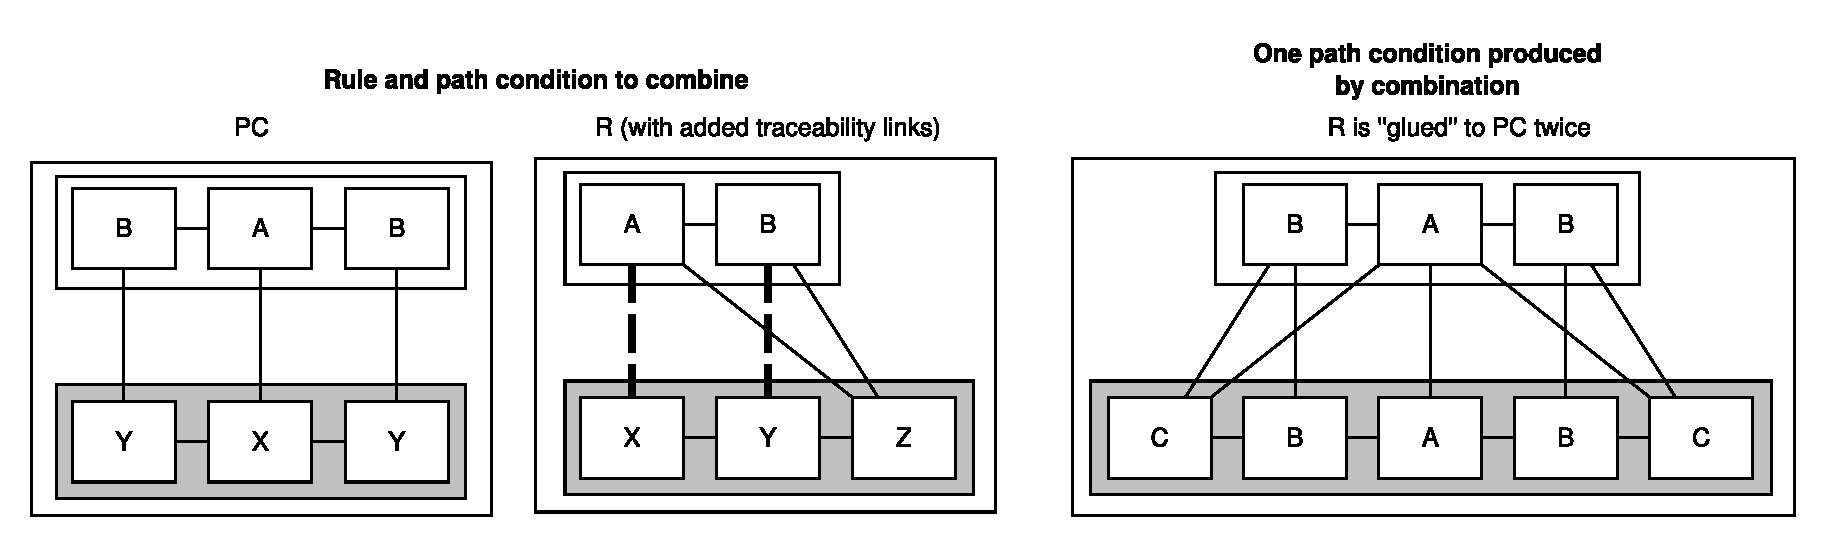
\includegraphics[width=1\textwidth]{./figures/building_path_conditions/multiple_total_satisfied_dependencies.pdf}
                \caption{Totally satisfied at multiple locations - \reviewer{Fix boxes on bottom}}
                \label{fig:multiple_total_satisfied_dependencies}
        \end{subfigure}%
        \caption{R's dependencies are totally satisfied by PC}
        \label{fig:totes_sat_deps}
\end{figure*}

In the partially-satisfied case, rule R may or may not execute. Note that in \cref{fig:partial_satisfied_dependencies}, PC does not have the association between the A and B elements in the match graph. This means that it is possible that the input model for the transformation does not have this association present. In these transformation executions R would not execute.
\cref{fig:partial_satisfied_dependencies} shows the two path conditions produced in this case. The first produced is a copy of PC, where R does not symbolically execute. The second is where R symbolically executes at the matched location. Therefore, R is glued onto PC, with the gluing step the same as in the totally-satisfied case above.

\begin{figure*}[tb] \centering 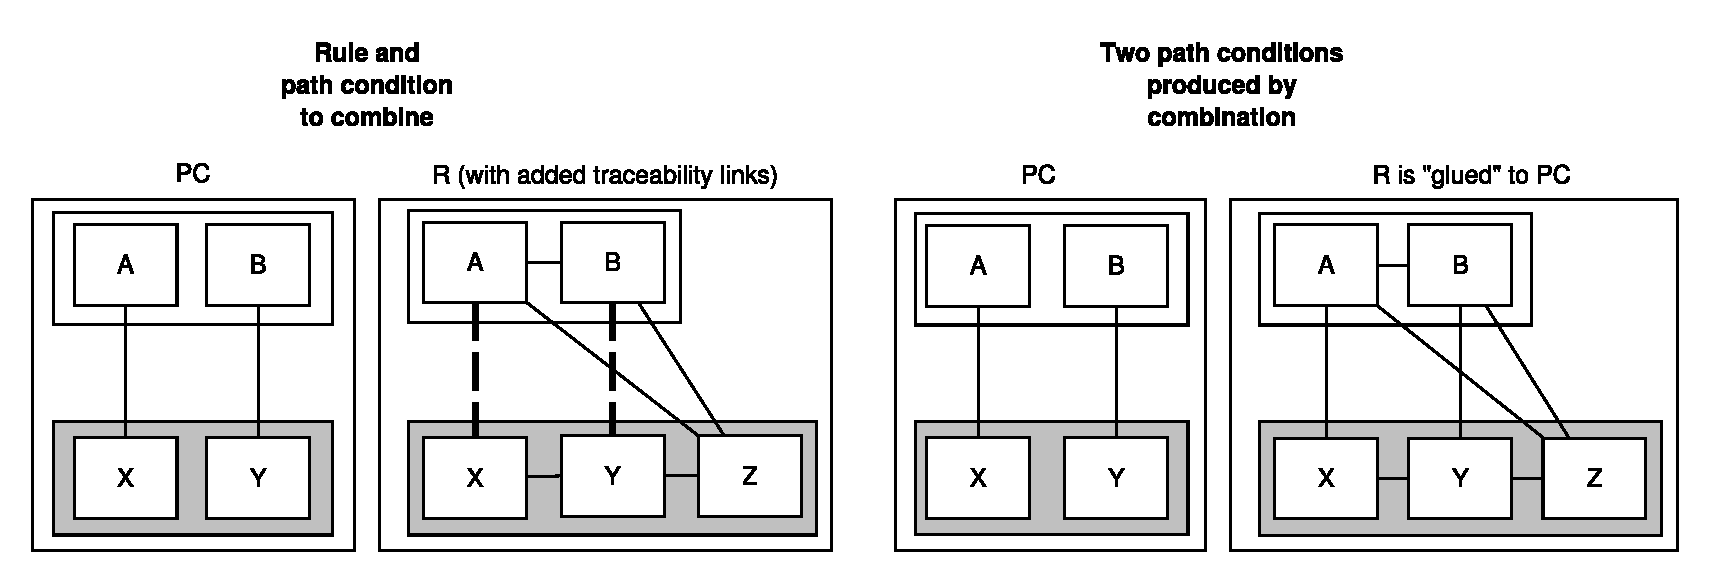
\includegraphics[width=0.8\textwidth]{./figures/building_path_conditions/partial_satisfied_dependencies.pdf}
	\caption{R's dependencies are partially satisfied by PC}
	\label{fig:partial_satisfied_dependencies}
\end{figure*}

Note that this gluing procedure must consider all matching possibilities, for each location the rule might match over the input model. For example, in \cref{fig:multiple_partial_satisfied_dependencies}, rule R has a backward link that can be partially matched on two locations in PC: the left-hand and right-hand pairs of traceability links. Therefore, there are four possibilities for how R would match over PC: not at all, on the left-hand side of PC, on the right-hand side, or on both sides. These four possibilities define the four new path conditions created.

The first is a copy of PC, as R is assumed to not execute and will produce no new elements. The second is where R will be glued on top of the backward links on the left-hand side, to add the elements that do not exist in PC already. The third is where the gluing will occur on the right-hand side. The fourth path condition produced is the case where R will be glued at both locations. 


\begin{figure*}[tb] \centering 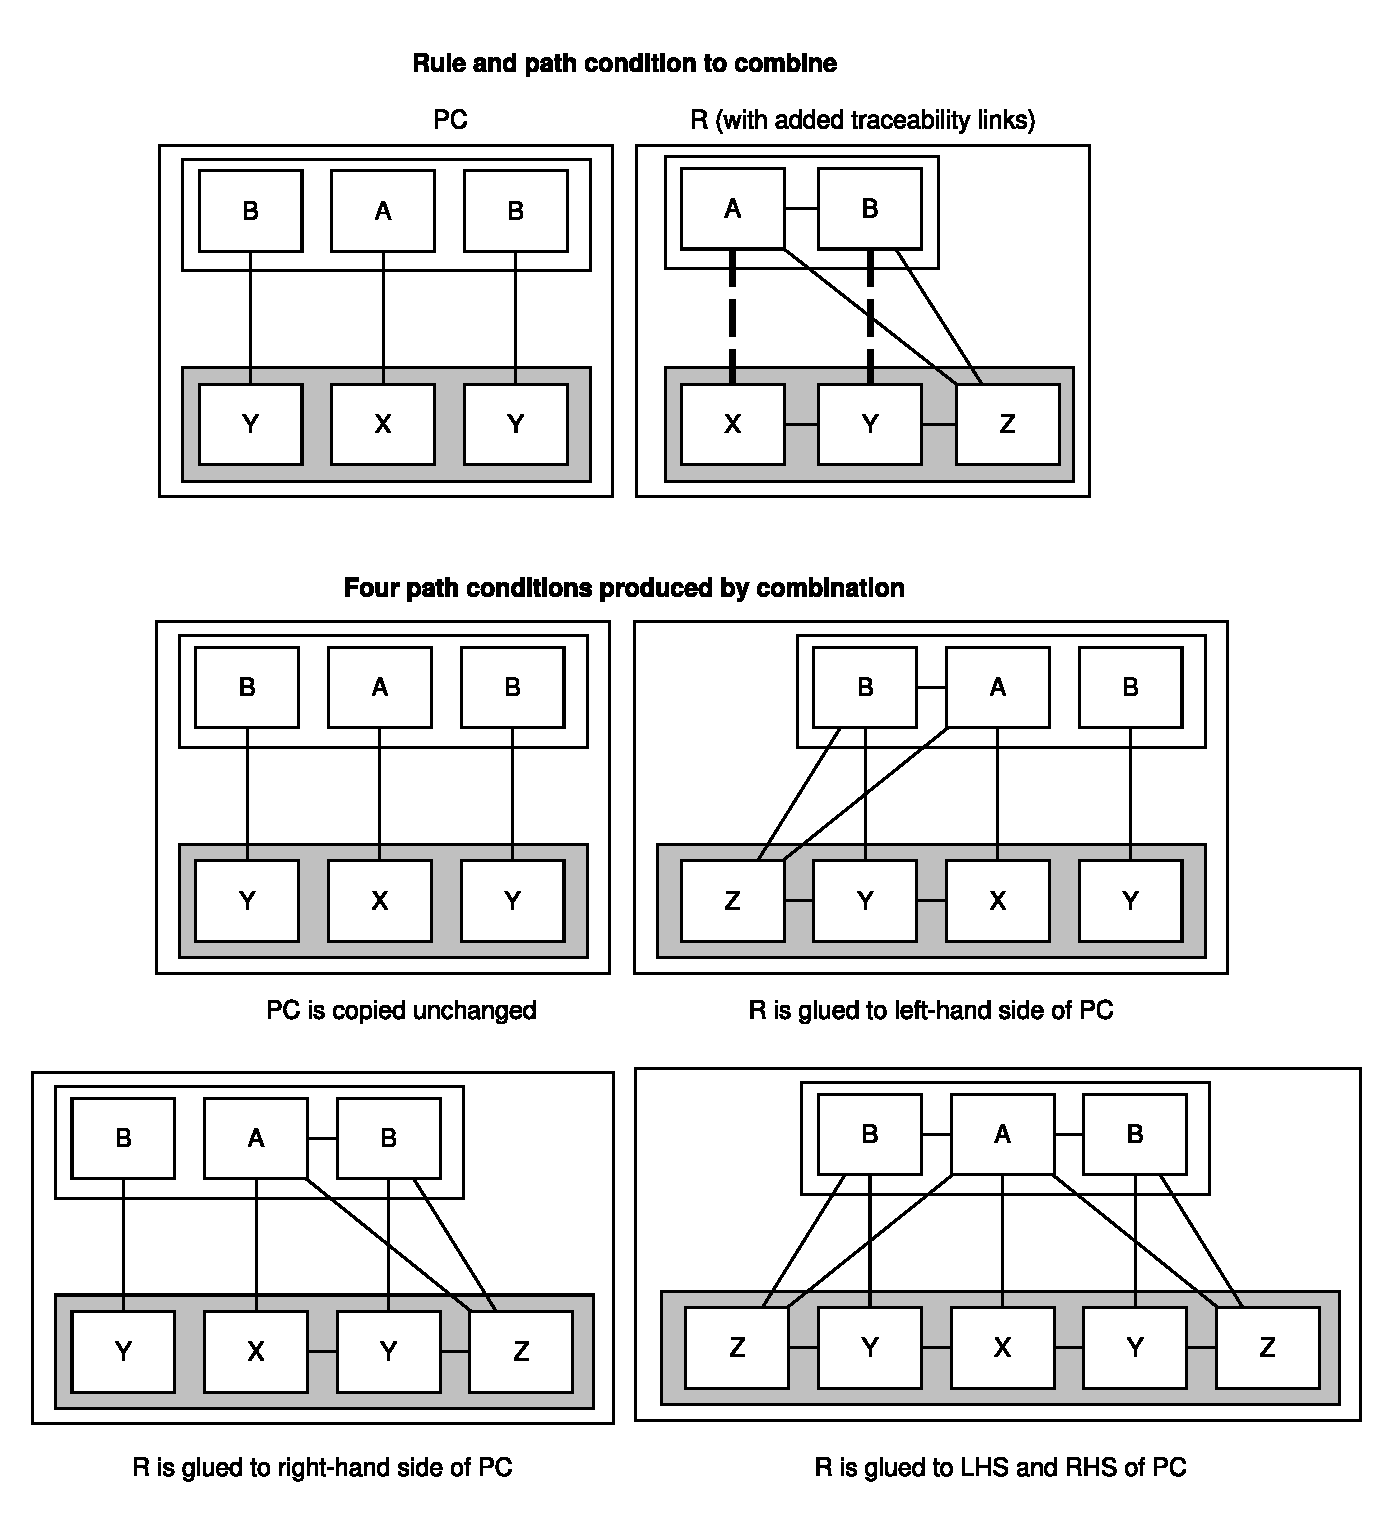
\includegraphics[width=0.8\textwidth]{./figures/building_path_conditions/multiple_partial_satisfied_dependencies.pdf}
	\caption{R's dependencies are partially satisfied by PC, and are glued at all possible matches}
	\label{fig:multiple_partial_satisfied_dependencies}
\end{figure*}


Note that rules may also contain transitive links in their match graphs. In this case, the partial or total matching of R onto PC must consider all transitive matches in order to produce all valid path conditions.

As we have done for the previous cases, let us now formally define the combination step when a rule has partially and/or totally defined dependencies. As these cases are more complex than the previous two, we will need to construct the mathematical model of this case incrementally. We will start by an auxiliary relation that partially or totally combines a set of path conditions with a rule.

\begin{definition}{Single Partial and Total Combination of a Set of Path Conditions with a Rule\\}
\label{def:comb_path_cond_rule_single}
% \begin{definition}{Satisfied Dependencies Between Two Path Conditions}
% 
% Let $A=\langle V_A,E_A,st_A,\tau_A,Match_A,Apply_A\rangle, B=\langle V_B,E_B,st_B,\tau_B,Match_B,Apply_B\rangle\in \textsc{Pathcond}^{sr}_{tg}$ be two path conditions. We say that $A$ satisfies $B$'s dependencies if and only if  $B'\vartriangleleft A'$, where $A'=A_{|backward}$ and $B'=B_{|backward}$.
% \end{definition}
% 
% A path condition A partially satisfies the dependencies of a path condition B if
% there exists an injective typed graph homomorphism between the backward links of
% B and those of A. In other words, 
%
% Note that this works for both cases where more instances of
% the same backward link exist in A, or in B.





The single rule partial and total combination relations $\stackrel{p\_comb}{\rightarrow}$ and $\stackrel{t\_comb}{\rightarrow}$, both having having signature $\mathcal{P}(\textsc{Pathcond}^{sr}_{tg}) \times \textsc{Rule}^{sr}_{tg} \times \textsc{Rule}^{sr}_{tg} \times \mathcal{P}(\textsc{Pathcond}^{sr}_{tg})$ are defined as follows:


\begin{align}
\label{eq:pcomb}
\frac{\begin{array}{ll}
rl\cong rl_{glue}\sqcup ma_{\Delta}
\end{array}}
{\langle AC,rl,rl_{glue}\rangle \xrightarrow{p\_comb} AC\;\;\cup\;\; \bigcup_{pc\in AC} pc\stackrel{trace}{\sqcup} (rl_{glue} \sqcup ma_{\Delta})}
\end{align}


\begin{align}
\label{eq:tcomb}
\frac{\begin{array}{ll}&
rl\cong rl_{glue}\sqcup ma_{\Delta}
\end{array}}
{\langle AC,rl,rl_{glue}\rangle \xrightarrow{t\_comb} \bigcup_{pc\in AC} pc\stackrel{trace}{\sqcup} (rl_{glue} \sqcup ma_{\Delta})}
\end{align}

\end{definition}


Let us start by introducing relation $\stackrel{p\_comb}{\rightarrow}$, presented in \cref{eq:pcomb} of \cref{def:comb_path_cond_rule_single}. The relation takes as arguments a set of path conditions being accumulated for the current layer, the rule to be combined, and an $rl_{glue}$ argument indicating the place in each of the input path conditions the rule should be anchored to during the combination step. The relation's output is a new set of path conditions. This new set includes all the original path conditions, as well as each path condition in the accumulator set ``glued'' to a copy of rule being examined. Note that the relation $\stackrel{t\_comb}{\rightarrow}$ in \cref{eq:tcomb} of \cref{def:comb_path_cond_rule_single} is similarly defined, except for the fact path conditions in the accumulator set are not preserved in the relation's output set.\\

\setcounter{equation}{0} 

Let us now define how a rule is combined with a path condition, whenever its backward links can be found several times in that path condition. This situation is described in the examples in \cref{fig:multiple_total_satisfied_dependencies} and \cref{fig:multiple_partial_satisfied_dependencies}. We formalize it in \cref{def:comb_path_cond_rule_mul}, by means of relations $\stackrel{p\_step}{\rightarrow}$ and $\stackrel{t\_step}{\rightarrow}$. These two relations operationally describe the sequence of steps necessary to ``glue'' a rule at multiples places of a path condition. The set of places targeted in the path condition for receiving a copy of the rule is given by the sets $partialSet$ and $totalSet$ (found respectively in Equation~(2) and Equation~(4) of \cref{def:comb_path_cond_rule_mul}). As expected, these sets contain the set of traceability links in the path condition where copies of the rule need to be anchored to.

\begin{definition}{Multiple Partial and Total Combination of a Set of Path Conditions with a Rule\\}
\label{def:comb_path_cond_rule_mul}



The multiple rule partial and total combination relations $\stackrel{p\_step}{\rightarrow}$ and $\stackrel{t_step}{\rightarrow}$, both having having signature $\mathcal{P}(\textsc{Pathcond}^{sr}_{tg}) \times \mathcal{P}(\textsc{Rule}^{sr}_{tg}) \times \textsc{Rule}^{sr}_{tg} \times \mathcal{P}(\textsc{Pathcond}^{sr}_{tg})$ are defined as follows:

\begin{align}
\label{eq:pstepbase}
\frac{\begin{array}{ll}
\end{array}}
{\langle AC,rl,\emptyset\rangle \xrightarrow{p\_step} AC}
\end{align}

\begin{align}
\label{eq:pstep}
\frac{\begin{array}{ll}
rl_{glue}\in &partialSet,\;\langle AC,rl,rl_{glue}\rangle \xrightarrow{p\_comb} AC''\;,\;\\
&\langle AC'',rl,partialSet\setminus\{rl_{glue}\}\rangle \xrightarrow{p\_step} AC'
\end{array}}
{\langle AC,rl,partialSet\rangle \xrightarrow{p\_step} AC'}
\end{align}

\begin{align}
\label{eq:tstepbase}
\frac{\begin{array}{ll}
\end{array}}
{\langle AC,rl,\emptyset\rangle \xrightarrow{t\_step} AC}
\end{align}

\begin{align}
\label{eq:tstep}
\frac{\begin{array}{ll}
rl_{glue}\in &totalSet\;,\;\langle AC,rl,rl_{glue}\rangle \xrightarrow{t\_comb} AC''\;,\;\\
&\langle AC'',rl,totalSet\setminus\{rl_{glue}\}\rangle \xrightarrow{t\_step} AC'
\end{array}}
{\langle AC,rl,totalSet\rangle \xrightarrow{t\_step} AC''} 
\end{align}
\end{definition}

Having \cref{def:comb_path_cond_rule_single} and \cref{def:comb_path_cond_rule_mul} in mind, we can now proceed to define the complete combination relation of a rule with a path condition in the case of partially and totally satisfied dependencies. 

\begin{definition}{Path Condition and Rule Combination -- Partially and Totally Satisfied Dependencies\\}
\label{def:rul_comb_partial_total}



% When a rule is combined with a path condition, partial and total matches of the rule may exist in the path condition. A total match of the rule is found in the path condition if a surjective typed graph homomorphism exists between the backward matcher of the rule and a subgraph of the path condition ($rl_{glue}\sqsubseteq pc \,\land\, rl\blacktriangleleft rl_{glue}$). As a reminder, the backward matcher of a rule consists of the rule's match part, together with its backward links (see \cref{def:back_match_transformation_rule}). In this case, existing path conditions in the output set will combined with\ldots
% 
% These two cases are modeled by the two inference rules in \cref{def:comb_path_cond_rule}. 
% 
% For each case a delta is added to the glue graph found such that the necessary apply or match part of the rules are added to the original path condition. In case the match is partial, then the previous set of path conditions is kept where the delta has been added, as well a second possibility with the total rule. Note that the fact that we use a surjective homomorphism allows us to deal with both rules that are isomorphic or homomorphic to parts of PC. This allows us to have more backward links in the path condition than in a rule, but also the other way around.



The combination of a path condition $pc$ and a rule $rl$, when $rl$ has dependencies that are satisfied by $pc$, is described by the relation $\stackrel{combine}{\rightarrow}\subseteq \textsc{Pathcond}^{sr}_{tg} \times \mathcal{P}(\textsc{Pathcond}^{sr}_{tg}) \times \textsc{Rule}^{sr}_{tg} \times \mathcal{P}(\textsc{Pathcond}^{sr}_{tg})$, defined as follows:%\levi{surjection is used too loosely here}	

% $$\frac{\begin{array}{ll}&
% pc\in PC\;,\;\langle pc,rl\rangle \xrightarrow{combine} pc'\;,\;PC\setminus\{pc\},rl,\rangle \xrightarrow{combstep} PC'
% \end{array}}
% {\langle PC,rules\rangle \xrightarrow{rulestep} PC'}$$

$$\frac{\begin{array}{ll}rl|_{trace}\blacktriangleleft &pc|_{trace}\;,\\&\langle AC,rl,partialsat(rl,pc)\rangle\xrightarrow{p\_step} AC''\;,\;\\&\langle AC'',rl,totalsat(rl,pc)\rangle \xrightarrow{t\_step} AC'
\end{array}} 
{\langle pc,AC,rl\rangle \xrightarrow{combine} AC'}$$
\begin{center}
\vspace{.3cm}
where
\begin{align*}
rl_{glue}\in&~partialsat(rl,pc) \;\Longleftrightarrow\; \\
&rl_{glue}\sqsubseteq pc^{*} \,\land\, rl|_{trace}\blacktriangleleft rl_{glue}\quad\land\, \\&\hspace{1cm}\nexists rl' \,.\, (rl_{glue}\sqsubseteq rl'\sqsubseteq pc^{*} \land \Vert rl\Vert \blacktriangleleft rl')
\end{align*}
and 
\begin{align*}
rl_{glue}\in totalsat(rl,pc) \;\Longleftrightarrow \;rl_{glue}\sqsubseteq pc^{*} \,\land\, \Vert rl\Vert\blacktriangleleft rl_{glue}
\end{align*}
\end{center}


\end{definition}

\reviewer{Def. 24: it seems to me you are making a very serious mistake here. $\blacktriangleright$ tests
for the existence of a morphism, but in Def. 19 you are relying on coincident node/edge identities. (See my remark 15.) Maybe you mean that the morphism from rl to pc should drive the choice of node/edge identity in the isomorphic copy of rl to be combined with pc, but this is really a wild guess on my part.}


The top equation in \cref{def:rul_comb_partial_total} defines the $\stackrel{combine}{\rightarrow}$ relation for when rule $rl$ has dependencies that are satisfied by path condition $pc$. The pre-conditions in the equation state that the backward links in the rule are found in the path condition, as expected. Additionally, two sequential steps perform the gluing of the rule $rl$ on all path conditions in accumulator $AC$, wherever the rule is partially and/or totally found in each of those path conditions. Relations $\stackrel{p\_comb}{\rightarrow}$ and $\stackrel{t\_comb}{\rightarrow}$ presented in \cref{def:comb_path_cond_rule_mul} are used to model these two operational ``gluing'' steps. Functions $partialsat$ and $totalsat$, described in the latter part of \cref{def:rul_comb_partial_total}, are used to gather the places of path condition $pc$ where copies of the rule need to be anchored to.


\subsubsection{Considering Further Rules}
\label{sec:further_rules}
Thus far we have described how to create a set of path conditions that represent how one rule from a layer will add new elements to one path condition from the previous layer. These path conditions are then themselves combined with the next rule in the layer in the same manner. Note that in \cref{def:rul_comb_partial_total} the choice of next rule does not matter, due to the rule non-interference guaranteed by the semantics of DSLTrans. In order to represent this non-interference in the construction of path conditions, we specify that the matching of rule dependencies is against the path condition from the previous layer (variable $pc$ in the main equation of \cref{def:rul_comb_partial_total}), not the specific path condition the rule is to be combined with in the accumulator argument of the $\stackrel{combine}{\rightarrow}$ relation. This ensures that the result of combining one rule with a path condition will have no impact on how following rules will combine.

% Note that the choice of next rule does not matter, due to the rule non-interference guaranteed by the semantics of DSLTrans. In order to represent this non-interference in the construction of path conditions, we specify that the matching of rule dependencies is against the path condition from the previous layer, not the specific path condition the rule is to be combined with. This ensures that the result of combining one rule with a path condition will have no impact on how following rules will combine.

The combination of one path condition with all the rules in the layer will produce a new set of path conditions. This process is depicted in \cref{fig:all_pcs2} and formalized in \cref{def:path_cond_layer_comb} by the layer combination relation $\stackrel{combpclayer}{\rightarrow}$.

\begin{definition} {Combining a Path Condition with a Layer\\}
\label{def:path_cond_layer_comb}

The \emph{layer combination relation}
$\stackrel{combpclayer}{\rightarrow}\subseteq \textsc{Pathcond}^{sr}_{tg} \times\\ \mathcal{P}(\textsc{Pathcond}^{sr}_{tg}) \times \textsc{Layer}^{sr}_{tg}\times
\mathcal{P}(\textsc{Pathcond}^{sr}_{tg})$ relation is defined as follows:
$$\frac{}
{\langle pc,AC,\emptyset\rangle \xrightarrow{combpclayer} AC}$$

$$\frac{\begin{array}{ll}rl\in layer,\;\langle pc,AC&,rl\rangle\xrightarrow{combine}AC'',\\ &\langle pc,AC'',layer\setminus\{rl\}\rangle\xrightarrow{combpclayer}AC'
\end{array}}
{\langle pc,AC,layer\rangle \xrightarrow{combpclayer} AC''}$$

\end{definition}

After the step in~\cref{def:path_cond_layer_comb} is repeated for all the path conditions in the previous layer, these new sets of path conditions are collected together to produce the working set of path conditions for the layer. This process is modeled by relation $\stackrel{combpcsetlayer}{\rightarrow}$ in \cref{def:path_cond_set_layer_comb}.

\begin{definition} {Combining a Set of Path Conditions with a Layer\\}
\label{def:path_cond_set_layer_comb}
The \emph{path condition layer step relation}
$\stackrel{combpcsetlayer}{\rightarrow}\subseteq \\\mathcal{P}(\textsc{Pathcond}^{sr}_{tg}) \times \textsc{Layer}^{sr}_{tg}\times
\mathcal{P}(\textsc{Pathcond}^{sr}_{tg})$ relation is defined as follows:
$$\frac{}
{\langle \emptyset,layer\rangle \xrightarrow{combpcsetlayer} \emptyset}$$

$$\frac{\begin{array}{ll}pc\in AC,\;\langle pc,\{pc\}&,layer\rangle\xrightarrow{combpclayer}AC',\\ &\langle AC\setminus\{pc\},layer\rangle\xrightarrow{combpcsetlayer}AC''
\end{array}}
{\langle AC,layer\rangle \xrightarrow{combpcsetlayer} AC'\cup AC''}$$
\end{definition}

This working set of path conditions obtained for each layer is then itself combined with the rules in the next layer as in the algorithm just described, to obtain yet another working set of path conditions. This process will then continue in this layer-by-layer fashion through the transformation and is formally described in \cref{def:path_cond_gen}.\\
After all layers have been processed, the working set of the last layer contains all the  possible path conditions of the transformation. Through our abstraction relation defined in \cref{sec:abstraction_relation}, the final set of created path conditions will represent every feasible transformation execution. \cref{sec:verif_dsltrans_props} will discuss how our algorithm proves properties on these path conditions, and thus on all executions of the transformation.

\begin{definition} {Path Condition Generation\\}
\label{def:path_cond_gen}
Let $[layer::tr]\in \textsc{Transf}^{sr}_{tg}$ be a transformation, where $layer\in
\textsc{Layer}^{sr}_{tg}$ is a Layer and $tr$ also a transformation. The $\stackrel{pathcondgen}{\rightarrow}\subseteq \mathcal{P}(\textsc{Pathcond}^{sr}_{tg}) \times \textsc{Transf}^{sr}_{tg}\times
\mathcal{P}(\textsc{Pathcond}^{sr}_{tg})$ is defined as follows:
$$\frac{}
{\langle AC,[\;]\rangle \xrightarrow{pathcondgen} AC}$$

$$\frac{\begin{array}{ll}\langle \epsilon_{pc},layer^{\star}\rangle\xrightarrow{combpcsetlayer}AC''\;,\;\langle AC'',tr\rangle\xrightarrow{pathcondgen}AC'
\end{array}}
{\langle \epsilon_{pc},[layer::tr]\rangle \xrightarrow{pathcondgen} AC}$$
$$\text{where } layer^{\star}=\bigcup_{rl\in l}rl^{\star}$$

\end{definition}

Note that in \cref{def:path_cond_gen}, the recursive rule considers the expansion ($layer^{\star}$) of all the rules in a layer (see \cref{def:transformation_rule_expansion}). This allows us to deal with polymorphism during path condition generation. In particular, given one rule $rl$ of $layer$, we consider for path condition generation all rules containing possible of replacements of each match element in $rl$ of certain type by an element belonging to one of the type's subtypes, as defined in the source metamodel $sr$.\\
After all layers have been processed, the working set of the last layer contains all the possible path conditions of the transformation. Through our abstraction relation in \cref{def:abstraction_pc_ex_appendix}, the final set of created path conditions will represent every feasible transformation execution.

\paragraph{\textbf{Notation:}}

We will use the abbreviation $\textsc{Pathcond}(tr)$ to represent the set of path conditions $AC$ produced for a transformation $tr$, where $\langle \epsilon_{pc},tr\rangle \xrightarrow{pathcondgen} AC$.





